\documentclass[tikz, border=10pt]{standalone}
\usetikzlibrary{shapes.geometric, arrows.meta, positioning, calc, shapes.multipart}

\begin{document}
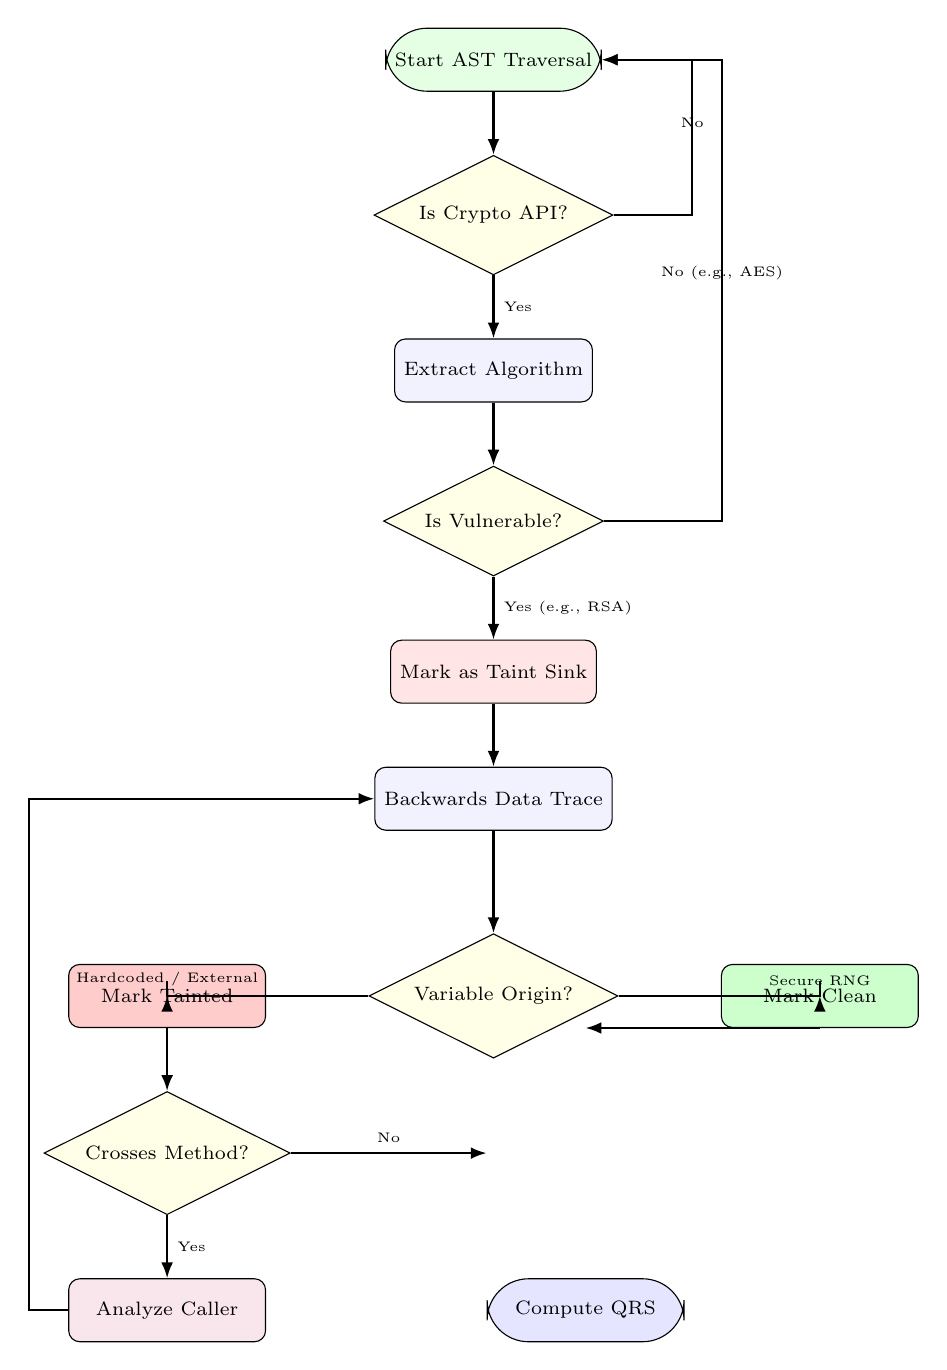
\begin{tikzpicture}[
    node distance=0.8cm and 0.8cm,
    box/.style={draw, rectangle, rounded corners, minimum width=2.5cm, minimum height=0.8cm, align=center, font=\scriptsize, fill=blue!5},
    decision/.style={draw, diamond, aspect=2, minimum width=2.5cm, minimum height=0.8cm, align=center, font=\scriptsize, fill=yellow!10},
    arrow/.style={thick, -{Latex[length=2mm]}}
]
    \node[box, rounded corners=15pt, fill=green!10] (start) {Start AST Traversal};
    \node[decision, below=of start] (iscrypto) {Is Crypto API?};
    \node[box, below=of iscrypto] (extract) {Extract Algorithm};
    \node[decision, below=of extract] (isvuln) {Is Vulnerable?};
    \node[box, below=of isvuln, fill=red!10] (marksink) {Mark as Taint Sink};
    \node[box, below=of marksink] (trace) {Backwards Data Trace};
    \node[decision, below=of trace, yshift=-0.5cm] (issource) {Variable Origin?};
    
    \node[box, left=of issource, xshift=-0.5cm, fill=red!20] (tainted) {Mark Tainted};
    \node[box, right=of issource, xshift=0.5cm, fill=green!20] (clean) {Mark Clean};
    
    \node[decision, below=of tainted] (crosses) {Crosses Method?};
    \node[box, below=of crosses, fill=purple!10] (caller) {Analyze Caller};
    
    \node[box, rounded corners=15pt, right=of caller, xshift=2cm, fill=blue!10] (qrs) {Compute QRS};

    \draw[arrow] (start) -- (iscrypto);
    \draw[arrow] (iscrypto) -- node[right, font=\tiny] {Yes} (extract);
    \draw[arrow] (iscrypto.east) -- ++(1,0) |- node[near start, above, font=\tiny] {No} (start.east);
    
    \draw[arrow] (extract) -- (isvuln);
    \draw[arrow] (isvuln) -- node[right, font=\tiny] {Yes (e.g., RSA)} (marksink);
    \draw[arrow] (isvuln.east) -- ++(1.5,0) |- node[near start, above, font=\tiny] {No (e.g., AES)} (start.east);
    
    \draw[arrow] (marksink) -- (trace);
    \draw[arrow] (trace) -- (issource);
    
    \draw[arrow] (issource) -| node[above, font=\tiny] {Hardcoded / External} (tainted);
    \draw[arrow] (issource) -| node[above, font=\tiny] {Secure RNG} (clean);
    
    \draw[arrow] (tainted) -- (crosses);
    \draw[arrow] (crosses) -- node[right, font=\tiny] {Yes} (caller);
    \draw[arrow] (caller.west) -- ++(-0.5,0) |- (trace.west);
    
    \draw[arrow] (crosses.east) -- node[above, font=\tiny] {No} (qrs.west |- crosses.east);
    \draw[arrow] (clean.south) -- (qrs.north |- clean.south);

\end{tikzpicture}
\end{document}
